
Three different frameworks are used during this study, which are \texttt{InferPy}, \texttt{BayesPy} and \texttt{Scikit-Learn}. The first two are specifically designed to probabilistic modeling whereas the last one is a general machine learning library. For this reason, we are briefly describing the usage of the first two and only explaining the functions we are using on the last, but, before briefly describing their usage, the study's file structure and used database are described.

Each study is made in a different file, available in both a \texttt{Jupyter Notebook (.ipynb)} and \texttt{Python script (.py)} using the name format \texttt{[model]\_[framework]\_[database]}. Apart from these, there are three main auxiliary files:

\begin{itemize}
  \item \texttt{packages}: This file contains a list of the installed packages. These packages might be installed using \texttt{pip install -r packages}.
  \item \texttt{models.py}: In this \texttt{Python} file, all parametric and variational models from \texttt{InferPy} are defined. This includes PCA, NLPCA and VAE.
  \item \texttt{functions.py}: In this file, all auxiliary functions are defined. The aim of these functions is either to make graphic representations or summarize the inference results.
\end{itemize}

Two different databases are used:
\begin{itemize}
  \item \texttt{Mnist}: a largely used dataset on a set of handwritten digits.
  \item \texttt{Breast Cancer Wisconsin}: characteristics of the cell nuclei present in breast mass.
\end{itemize}

\subsection{Mnist}

\texttt{Mnist} database can be directly obtained through \texttt{InferPy.data}. It consists of a set of \(70.000\)  handwritten digits, codified as \(28\times 28\) binary matrices (Figure~\ref{fig:mnist_example} shows an example of digits within the database). Given this, the observed data belongs to \(\{0,1\}^{784}\). Each sample is labeled with its corresponding digit.

\begin{figure}[h!]
    \centering
    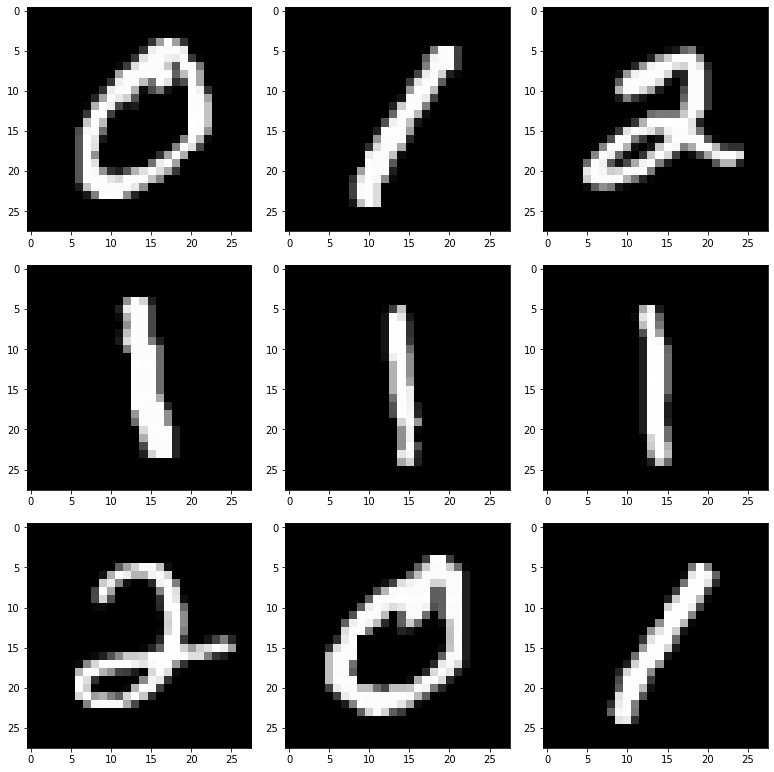
\includegraphics[width=0.35\textwidth]{tex/images/mnist.png}
    \caption{Mnist dataset example.}\label{fig:mnist_example}
\end{figure}

\subsection{Breast cancer Wisconsin}

\texttt{Breast cancer} database can be obtained from its \texttt{UCI} (\cite{DUA:2019}) repository \href{https://archive.ics.uci.edu/ml/datasets/Breast+Cancer+Wisconsin+(Diagnostic)}{link}. The database consists of \(569\) instances of \(30\) features of the cell nuclei present in breast mass. Among with each instance, an ID number and the diagnosis (\( M = \text{malign}\) and \(B = \text{benign}\)) are given. The given attributes are mean, standard error and worst (largest) value of all cells of the following features:
\begin{itemize}
  \item Radius: mean distance from the center to the perimeter.
  \item Texture: standard deviation of gray-scale values.
  \item Perimeter.
  \item Area.
  \item Smoothness: local variation in radius length.
  \item Compactness: \(perimeter^{2} / area - 1\).
  \item Concavity: severity of concave portions of the contour.
  \item Concave points: number of concave portions of the contour.
  \item Symmetry.
  \item Fractal dimension: a ratio comparing how detail in a fractal pattern changes with the scale of measurement.
\end{itemize}
All these features are coded with four significant digits.
